\def\tutdate{29.11.2018}

\documentclass[handout]{beamer}
\usepackage{../templates/beamerthemekitwide}
%\usepackage{enumitem}

\usepackage[utf8]{inputenc}
\usepackage[T1]{fontenc}
\usepackage[ngerman]{babel}
\usepackage{listings}
\usepackage{hyperref}
\usepackage{graphicx}

\usepackage{amsmath}
\usepackage{amsthm}
\usepackage{amssymb}
\usepackage{polynom}

%\usepackage{ifthen}
%\usepackage{adjustbox} % for \adjincludegraphics

%\usepackage{tikz}
\usepackage{listings}

%\usepackage[]{algorithm2e}

%\usepackage{colortbl}
\usepackage{verbatim}
%\usepackage{alltt}
%\usepackage{changes}

%\usepackage{pdfpages}
%\usepackage{tabularx}

%\usepackage{euler}


\newcommand{\markBlue}[1]{\textcolor{kit-blue100}{#1}}
\newcommand{\markGreen}[1]{\textcolor{kit-green100}{#1}}
\newcommand{\vertspace}{\vspace{.2cm}}

%\newcommand{\#}{\markBlue{#1}}

%\newcommand{\pitem}{\pause\item}
\newcommand{\p}{\pause}

% -- MATH MACROS
\newcommand{\thistheoremname}{}
\newcommand{\G}{\mathbb{Z}}
\newcommand{\B}{\mathbb{B}}
\newcommand{\R}{\mathbb{R}}
\newcommand{\N}{\mathbb{N}}
\newcommand{\Q}{\mathbb{Q}}
\newcommand{\C}{\mathbb{C}}
\newcommand{\Z}{\mathbb{Z}}
\newcommand{\F}{\mathbb{F}}
\newcommand{\mi}{\mathrm{i}}
\renewcommand{\epsilon}{\varepsilon}
\newcommand{\okalk}{\mathscr{O}}


\newenvironment<>{taskblock}[1]{%
	\setbeamercolor{block title}{fg=kit-orange15,bg=kit-orange100}
	\setbeamercolor{block body}{fg=black,bg=kit-orange30}%
	\begin{block}#2{#1}}{\end{block}}

\setbeamertemplate{enumerate items}[default]

% Aussagenlogik Symbole
\newcommand{\W}{w}
\renewcommand{\F}{f}

% Kodierung
\newcommand{\frepr}{\textbf{repr}}
\newcommand{\fRepr}{\textbf{Repr}}
\newcommand{\fZkpl}{\textbf{Zkpl}}
\newcommand{\fbin}{\textbf{bin}}
\newcommand{\fdiv}{\textbf{ div }}
\newcommand{\fmod}{\textbf{ mod }}

% Speicherabbild
\newenvironment{memory}{\begin{tabular}{r | l}Adresse&Wert\\\hline\hline}{\end{tabular}}
\newcommand{\memrow}[2]{#1 & #2 \\\hline}

% Praedikatenlogik
\newcommand{\objequiv}{\stackrel{\cdot}{=}}
\newcommand{\pval}{val_{D,I,\beta}}

% Neue Befehle
\newcommand{\ip}{\pause} % inline pause, für mitten im satz
\newcommand{\pitem}{\pause\item} % für aufzählungen
\newcommand{\bp}{\pause} % block pause, für zwischen blöcken
\title[Grundbegriffe der Informatik]{ICPC\\Gruppe 2}
\date{\tutdate}
\subtitle{\tutTitle}
\author{Elias Schaut, Dennis Kobert, Niklas Kniep, Lam Vo, Ilia Bozhinov}

\institute{}

\titleimage{bg}
%\titleimage{bg-advent}

%
\ifthenelse{\equal{\compiletype}{livebeamer}}
	{
		\def\livebeamermode{1}
	}{}

\ifthenelse{\equal{\compiletype}{print}}
	{
		\def\printmode{1}
	}{}

\setbeamercovered{invisible}

%\usepackage[citestyle=authoryear,bibstyle=numeric,hyperref,backend=biber]{biblatex}
%\addbibresource{templates/example.bib}
%\bibhang1em


\def\tutTitle{Kontextfreie Grammatiken, Relationen}
\begin{document}
	
	\selectlanguage{ngerman}
	
%title page
\begin{frame}
	\titlepage
\end{frame}

\section{Hinweise}

\begin{frame}
Erinnerung: Anmeldung für Klausur und Übungsschein im Campus System nicht vergessen!
\end{frame}

\begin{frame} {Häufige Fehler}
\begin{itemize}
	\item $w \in \{0, 1\}^*$
	\item nicht $w \geq 0$, sondern $Num_2 (w) \geq 0$ oder $w(0)=0$
	\pitem $f:A \rightarrow A^*$ induziert den Homomorphismus $f^{**}:A^* \rightarrow A^*$, ist aber selbst keiner
	\pitem $h:A^* \rightarrow A^*$ mit $\forall w \in A^*: h(w) = 0$ ist kein Homomorphismus. Warum nicht?
\end{itemize}
\end{frame}

\section{Kontextfreie Grammatiken}
\begin{frame}{Kontextfreie Grammatiken}
	Zur Rekapitulation...
	
	\begin{itemize}
		\pitem Was ist ein Alphabet, was eine formale Sprache?
		\pitem Was kennen wir für Operationen auf formalen Sprachen?
	\end{itemize}

	\bp 
	
	Betrachte $L := \{a^nba^n : n \in \N \}$. \ip Wie kann man diese Sprache darstellen?
\end{frame}

\begin{frame}{Kontextfreie Grammatiken}
	\begin{block}{Kontextfreie Grammatik}
		Ein Tupel G = (N, T, S, P) mit
		\begin{itemize}
			\item $N$ Alphabet (Nichtterminalsymbole)
			\item $T$ Alphabet mit $N \cap T = \emptyset$ (Terminalsymbole)
			\item $S \in N$ (Startsymbol)
			\item $P \subseteq N \times (N \cup T)^* \text{ mit } |P| \in \mathbb{N}_0$
		\end{itemize}
	\end{block}

	\begin{itemize}
		\pitem Was ist $N \times (N \cup T)^*$? Bei $T := \{a,b,c\}, N = \{S, A, B\}$\ip : $N \times (N \cup T)^* = \{(S, abSAcB), (A, SSS), (B, BSabc), ...\}$.
		\pitem Andere Schreibweise: $P : N \rightarrow (N \cup T)^*$.
		\pitem Für $(X, w) \in P$ schreibt man $X \rightarrow w$
		\pitem Statt $\{X\rightarrow w_1, X \rightarrow w_2 \}$ schreibt man auch $\{X \rightarrow w_1 | w_2\}$
	\end{itemize}
	
\end{frame}

\begin{frame}{Ableitungsschritt}
	Erinnerung: $N = Nichtterminalsymbole$, $T = Terminalsymbole$. \pause
	
	\begin{block}{Ableitungsschritt}
		$v \in (N \cup T)^*$ ist in einem Schritt aus $u \in (N \cup T)^*$ ableitbar , wenn 
		\begin{itemize}
			\pitem $u = w_1 X w_2 \text{ und } v = w_1 w_X w_2 \text{ für } w_1, w_2 \in (N \cup T)^* $
			\pitem und $X \rightarrow w_X$ in $P$
		\end{itemize}
	\end{block}

	\bp\markBlue{Notation}\\
	$u\Rightarrow v$\\
	\bp\markBlue{Beispiel}\\
	$G:= (\{S,B\}, \{a,b\}, S, \{S \rightarrow aBa|aSa, B \rightarrow b\})$
	
	\begin{itemize}
		\pitem $S \ip\Rightarrow aSa \ip\Rightarrow aaSaa \ip\Rightarrow aaaBaaa \ip\Rightarrow aaabaaa$. \ip Fertig.
		\pitem $aaaSaaa \not\Rightarrow aaaabaaaa$! 
		\pitem ``$\Rightarrow$'' heißt \markGreen{eine} Ableitung!
	\end{itemize}
\end{frame}

\begin{frame}{Ableitungsfolge}
	\begin{block}{Ableitungsfolge}
	    Wir definieren $\Rightarrow^i$ für $i \in \mathbb{N}_0$ folgendermaßen:\\\vspace{.3cm}
		\bp Für $u,v \in (N \cup T)^*$ gelte:
		\begin{itemize}
			\item $u \Rightarrow^0 v$ genau dann, wenn $u = v$ gilt.
			\item $u \Rightarrow^{i+1} v$ genau dann, wenn ein $w \in (N \cup T)^* $ existiert, für das $u \Rightarrow w \Rightarrow^i v$ gilt.
			Für $u \Rightarrow^i v$ sagt man \markGreen{``v ist aus $u$ in $i$ Schritten ableitbar.''}
		\end{itemize}
	\end{block}

	\bp

	\textbf{Beispiel}\\
	$G:= (\{S,B\}, \{a,b\}, S, \{S \rightarrow aBa|aSa, B \rightarrow b\})$\\
	\ip Dann gilt $aaaSaaa \Rightarrow^0 aaaSaaa$ \ip \\
	und $aaaSaaa \Rightarrow^2 aaaabaaaa$
\end{frame}

\begin{frame}
	\begin{block}{Ableitbarkeit}
		Für $u,v \in (N \cup T)^*$ gelte $u \Rightarrow^* v$ genau dann, wenn ein $i \in \mathbb{N}_0$ existiert , mit $u \Rightarrow^i v$. Man sagt dann \markGreen{``v ist aus u ableitbar''}.
	\end{block}\bp
	\textbf{Beispiel}\\
	$G:= (\{S,B\}, \{a,b\}, S, \{S \rightarrow aBa|aSa, B \rightarrow b\})$\\
	\ip Dann gilt $S \Rightarrow^* aaaSaaa$ \ip \\
	und $aSa \Rightarrow^* aaaabaaaa$ \ip \\
	aber $aSa \not\Rightarrow abba$.
\end{frame}

\begin{frame}{Ableitungsbaum}
	\begin{columns}
		\begin{column}{0.5\textwidth}
			\begin{itemize}
				\item Startsymbol ist Wurzel
				\item Nichtterminale sind innere Knoten
				\item Für $X \Rightarrow w $ sind die Zeichen von $w$ die Kinder von X
				\item Terminale sind die Blätter
			\end{itemize}
		\end{column}
		
		\begin{column}{0.5\textwidth}\bp
			\textbf{Beispiel}\\
			$G:= (\{S,B\}, \{a,b\}, S, \{S \rightarrow aBa|aSa, B \rightarrow b\})$\bp\\
			Dann gilt $S \Rightarrow^* aaabaaa$\\
			\center 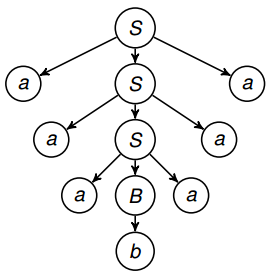
\includegraphics[scale=0.7]{images/Ableitungsbaum.png}
		\end{column}
	\end{columns}
	
\end{frame}

\begin{frame}{Übung zu Kontextfreien Grammatiken}
	\begin{taskblock}{Übung}
		Gegeben ist die Kontextfreie Grammatik (N, T, S, P) mit:
		
		\begin{itemize}
			\item Nichtterminalsymbolen $N := \{A, B, S\}$.
			\item Terminalsymbolen $T := \{a, b, c\}$
			\item Startsymbol $S$
			\item Produktionen $P := \{S \rightarrow aaS | bbS | SAS | \epsilon, A \rightarrow cB , B \rightarrow a | b| c | \epsilon\}$.
		\end{itemize}
	
		\bp
	
		Aufgabe: Welche der folgenden Wörter sind ableitbar? Konstruiere den Ableitungsbaum und zeige, wie sie abgeleitet werden.
		
		\begin{itemize}
			\item $ccbbcbbbbcbbaaaa$? %ja
			\item $aabbaabbaabb$? %ja
			\item $c$?
		\end{itemize}
	\end{taskblock}
\end{frame}

\begin{frame}{Formale Sprachen erzeugen}
	\begin{block}{Erzeugte Sprache}
		Sei $G = (N, T, S, P)$ eine kontextfreie Grammatik. Dann nennen wir $L(G) := \{w \in T^*| S \Rightarrow^* w\}$ die von G erzeugte Sprache.
	\end{block}

	\bp
	
	\begin{block}{Kontextfreie Sprache}
		Eine formale Sprache $L$ heißt genau dann kontextfrei, wenn eine kontextfreie Grammatik $G$ existiert, mit $L(G) = L$.
	\end{block}

	\bp

	$G:= (\{S,B\}, \{a,b\}, S, \{S \rightarrow aBa|aSa, B \rightarrow b\})$\\\vspace{.3cm}
	\ip Dann ist $L(G) = \{a^nba^n|n \in \mathbb{N_+}\}$
\end{frame}

\begin{frame}{Verständnisfragen}
	\begin{itemize}
		\item $G = (\{X\}, \{a,b\}, X, \{X \rightarrow \varepsilon| aX| bX\})$
		\begin{itemize}
			\item Welche Wörter lassen sich in genau drei Schritten ableiten?
			\pause		 		
			\item[$\rightarrow$] $\{aa, ab, ba, bb\}$
			\pause
			\item Was ist $L(G)$?
			\pause		 		
			\item[$\rightarrow$] $L(G) = \{a,b\}^*$
		\end{itemize}
		\pause
		\item Gibt es auch eine Grammatik $G$ mit $L(G) = \{\}$?
		\pause
		\item[$\rightarrow$] $G_1 := (\{X\}, \{a,b\}, X, \{X\rightarrow X\})$ oder $G_2 := (\{X\}, \{a,b\}, X, \{\})$
		\pause
		\item Wahr oder falsch? Wenn $w_1 \Rightarrow w_2$ gilt, dann gilt auch $w_1 \rightarrow w_2$
		\pause
		\item Was ist der Unterschied von $\Rightarrow$ und $\Rightarrow^*$ ?
	\end{itemize}
\end{frame}

\begin{frame}
	\begin{taskblock}{Aufgaben zu kontextfreien Grammatiken}
		\begin{itemize}
			\item Sei $L_1 := \{wbaaw'|w, w' \in \{a,b\}^*\}$. Konstruiere eine Grammatik $G_1$ mit $L(G_1) = L_1$.
			\pause
			\item[$\rightarrow$] $G_1 := (\{X, Y\}, \{a,b\}, X, \{X \rightarrow YbaaY, Y \rightarrow aY|bY|\varepsilon\})$.
			\pause
			\item  Welche Sprache erzeugt $ G_2 = (\{S, X, Y\}, \{a,b\}, S, P_2)$  mit $P_2 = \{S \rightarrow X|Y, X \rightarrow aaXb|aab, Y \rightarrow aYbb|abb\}$?
			\pause			
			\item[$\rightarrow$] $L(G_2) = \{a^{2k}b^{k} | k \in \mathbb{N}_+\} \cup \{a^kb^{2k}| k \in \mathbb{N}_+\}$
			%\pause
			%\item Sei $L_3 := \{w \in \{a,b\}^*| \forall \text{ Präfixe } v \text{ von } w : |N_a(v) - N_b(v)| \leq 1 \}$. Konstruiere eine Grammatik $G_3$ mit $L(G_3) = L_3$
			%\pause
			%\item[$\rightarrow$] $G_3 = (\{X\}, \{a,b\}, X, \{X\rightarrow abX|baX|a|b|\varepsilon\})$
		\end{itemize}
	\end{taskblock}	
\end{frame}

\begin{frame}{Beispiel zu kontextfreien Grammatiken}
	$G= (\{X\}, \{\textcolor{blue}{(}, \textcolor{blue}{)}\}, X, \{X \rightarrow XX|\textcolor{blue}{(} X \textcolor{blue}{)}| \varepsilon\} )$
	\begin{itemize}
		\item Welche Wörter sind ableitbar?
		\pause
		\item[$\rightarrow$] ``wohlgeformte Klammerausdrücke''
		\pause
		\item Welche Eigenschaften besitzen diese Wörter?
		\pause
		\item[$\rightarrow$]$N_{\textcolor{blue}{(}}(w) = N_{\textcolor{blue}{)}}(w)$ \pause Ist diese Eigenschaft hinreichend?
		\pause
		\item[$\rightarrow$]Nein, es muss gelten: Für alle Präfixe $v$ von $w$ gilt $ N_{\textcolor{blue}{(}}(v) \geq N_{\textcolor{blue}{)}}(v)$
		\pause
		\item Andere Grammatik möglich, die alle wohlgeformten Klammerausdrücke erzeugt?
		\pause
		\item[$\rightarrow$]  $G= (\{X\}, \{\textcolor{blue}{(}, \textcolor{blue}{)}\}, X, \{X \rightarrow \textcolor{blue}{(} X \textcolor{blue}{)}X| \varepsilon\} )$
	\end{itemize}
\end{frame}

\begin{frame}{Grenze kontextfreier Grammatiken}
	Es gibt auch Sprachen, die wir nicht mit einer kontextfreien Grammatik erzeugen können!
	
	\vspace{.3cm} \bp
	Beispiel aus der Vorlesung:\\
	$L_{vv} = \{vcv| v \in \{a,b\}^*\} \subseteq \{a, b, c\}^*$
\end{frame}


\section{Relationen vol. 2}
\begin{frame}{Relationen}
	\pause
	\begin{block}{Erinnerung Relationen}
		Es seien A und B Mengen. Eine Teilmenge $R \subseteq A \times B$ heißt Relation.
	\end{block}
\end{frame}

\begin{frame}	
	\begin{block}{Definition Produkt von Relationen}
		Es seinen $A, B \text{ und  } C$ Mengen und $R \subseteq A \times B, S \subseteq B \times C$ Relationen. Dann ist \\$S \circ R := \{(a,c) \in A \times C | \text{ } \exists b \in B \text{ mit } (a,b) \in R \land (b,c) \in S\}$ \\
		das Produkt der Relationen $R$ und $S$.
	\end{block}
	\bp\textbf{Bemerkung}\\
	\ip $S \circ R$ ist eine Relation auf $A$ und $C$\ip , bildet also von $A$ nach $C$ ab.
	\bp\begin{block}{Assoziativität des Produktes}
		Es seien $ A, B, C$ und $D$ Mengen und $R \subseteq A \times B, S \subseteq B \times C$ sowie $T \subseteq C \times D$ Relationen. 
		Dann gilt\ip \\
		$(T \circ S) \circ R = T \circ (S \circ R)$.
	\end{block}
\end{frame}

\begin{frame}
	\begin{block}{Homogene Relation}
		Es seien A und B Mengen und $R \subseteq A \times B$ eine Relation. $R$ heißt homogen, wenn $A=B$ und heterogen, wenn $A \neq B $ gilt.
	\end{block}
	
	\bp\begin{block}{Identität}
		Sei $M$ eine Menge. $I_M := \{(x,x)| x \in M\}$		
	\end{block}

	\bp\begin{block}{Potenz von Relationen}
		Sei $M$ eine Menge und $R \subseteq M  \times M$ eine homogene Relation. \ip Dann definieren wir $R^i$ für $i \in \mathbb{N}_0$ folgendermaßen: 
		\begin{itemize}
			\pitem $R^0 := I_M$
			\pitem Für alle $i \in \mathbb{N}_0: R^{i+1} := R^i \circ R$
		\end{itemize}
	
		\ip Also $R^4 = R \circ R \circ R \circ R$.
	\end{block}
\end{frame}

\begin{frame}{Reflexitivität}
	\bp\begin{block}{Satz über das neutrale Element}
		Es seien $A$ und $B$ Mengen und $R \subseteq A \times B$ eine Relation. Dann gilt: $R \circ I_B = R = I_A \circ R$.
	\end{block}
	
	\bp\begin{block}{Reflexivität}
		Sei M eine Menge und $R \subseteq M \times M$ eine homogene Relation. Wenn für alle $x \in M: (x,x) \in R$, nennt man $R$ reflexiv.
		
		\ip Also jedes Element der Definitionsmenge der Relation wird auf sich selbst abgebildet (und vielleicht auch auf andere Elemente abgebildet).
	\end{block}
	
	\bp\begin{block}{Lemma}
		Sei $M$ eine Menge und $R \subseteq M \times M$ eine homogene Relation. $R$ ist genau dann reflexiv, wenn $I_M \subseteq R$ gilt.
	\end{block}
\end{frame}

\begin{frame}{Transitivität}
	\bp\begin{block}{Transitivität}
		Sei $M$ eine Menge und $R \subseteq M \times M$ eine homogene Relation. \\ \ip R heißt transitiv, wenn: \ip\\ $\forall x, y, z \in M: (x,y) \in R \land (y, z) \in R \rightarrow (x,z) \in R$
	\end{block}
	
	\bp\begin{block}{Lemma}
		Sei $M$ eine Menge und $R \subseteq M \times M$ eine homogene Relation. $R$ ist genau dann transitiv, wenn $R \circ R \subseteq R$.
	\end{block}
\end{frame}

\begin{frame}
	\textbf{Aufgaben}\\
	Sei $M := \{1, 2, 3 \}$.
	\begin{itemize}
		\item Ist $R:= \{(1,1), (1,2), (2,3)\}$ transitiv? \pause Nein!
		\pause
		\item Ist $R$ reflexiv? \pause Nein!
		\pause
		\item Wie müsste R aussehen, um transitiv zu sein?
		\pause
		\item Ist $S:= \{(1,1), (1,2), (1,3), (2,2), (2,3)\}$ reflexiv? \pause Nein!
		\pause
		\item Ist $S$ transitiv? \pause \hspace{0.3cm} Ja!
		\item Wie müsste S aussehen, um reflexiv zu sein?
	\end{itemize}
\end{frame}

\begin{frame}{Reflexiv-transitive Hülle}
	\bp\begin{block}{Definition}
		Sei M eine Menge und $R \subseteq M \times M$ eine homogene Relation. \\Dann nennt man $R^* := \bigcup\limits_{i \in \mathbb{N}_0} R^i$ die reflexiv-transitive Hülle von R.
	\end{block}
	\bp\begin{block}{Satz}
		\begin{itemize}
			\item $R^*$ ist reflexiv
			\item $R^*$ ist transitiv
			\item $R^*$ ist die kleinste Relation, die reflexiv und transitiv ist und $R \subseteq R^*$ erfüllt.
		\end{itemize}
	\end{block}
	\bp\textbf{Bemerkung}\\
	\begin{itemize}
		\item Sei M eine Menge und $R\subseteq M \times M$ eine homogene, reflexive und transitive Relation. Dann gilt $R^* = R$.
	\end{itemize}
	
\end{frame}
\begin{frame}
	\textbf{Aufgaben}\\
	\begin{itemize}
		\item Sei $M = \{1, 2, 3\}$ und $R := \{(1,1), (1,2), (2,3)\}$ Was ist $R^*$?
		\pause
		\item[$\rightarrow$] $R^* = \{(1,1), (1,2), (1,3), (2,2), (2,3), (3,3)\}$ 
		\pause
		\item Sei $M$ eine Menge und $R \subseteq M \times M$ eine homogene Relation. Was ist $(R^*)^*$ ?
		\pause
		\item[$\rightarrow$]  $(R^*)^* = R^*$
		\pause
		\item $M := \{1,2,3,4\} \text{ und } R := \{(1,2), (2,3), (3,4), (4,1)\} \subseteq M \times M$. Ist R reflexiv? Ist R transitiv? \pause \hspace{0.3cm} Nein und nein!
	\end{itemize}
\end{frame}

\begin{frame}
	Die Relationen $R$ und $S$ über $\mathbb{N}_0$ seien gegeben durch:
	\begin{itemize}
		\item Für alle $a, b \in \mathbb{N}_0: aRb \Leftrightarrow a|b$ ($a$ ist Teiler von $b$)
		\item Für alle $a, b \in \mathbb{N}_0: aSb \Leftrightarrow ggT(a,b) = 1$ 
	\end{itemize}
	Prüfe auf Reflexivität und Transitivität!
	\pause
	\begin{itemize}
		\item[$\rightarrow$] R ist transitiv, aber nicht reflexiv.
		\pause
		\item[$\rightarrow$] S ist reflexiv, aber nicht transitiv.
	\end{itemize}
\end{frame}


\begin{frame}
	
\includegraphics[width=\linewidth]{../images/thatsall.png}
\end{frame}


\end{document}